%!TEX root = ../main.tex

\section{Conditional Diversification Benefit} % (fold)
\label{sec:conditional_diversification_benefit}

This section studies a new measure of diversification in a portfolio called \emph{conditional diversification benefit} (CDB), which is developed by \textcite{ChristoffersenErrunzaJacobLanglois2012}. CDB is based on the portfolio expected shortfall (ES), i.e. the expected loss in case the return materializes below a certain percentile, and therefore concerns the properties of the tail of the portfolio distribution. 

We begin by describing the construction and intuition of CDB and subsequently present the results of two analyses using CDB: First, we use simulated distributions of portfolio returns form our Student's \textit{t} dynamic copula model to discuss the relative diversification benefits of HML, CMA and RMW. Second, we compare the diversification benefits of out-of-sample investing according to one of three strategies: (1) mean-variance weights, (2) diversification optimal weights and (3) equal weights.

\subsection{Formula and interpretation of the CDB statistic}

If factors are not multivariate normal, the covariance matrix used in mean-variance optimization is not a full description of the dependency between factors. Factor returns are not normal, and therefore higher moments influence the tail behavior of their returns. These considerations are important for any portfolio looking to manage risk by diversifying across factors. The CDB measure gives an easy-to-interpret measure of how well diversified the tail of the portfolio return distribution is, for given portfolio weights.

Define ES as the expected loss in some bottom percentile $q$
\begin{align}
    \text{ES}_{i,t}^q(r_{i,t}) = -\mathbb{E}[r_{i,t} | r_{i,t} \leq F_{i,t}^{-1}(q)]
\end{align}
where $F_{i,t}^{-1}(q)$ is the inverse CDF of simple returns $r_{i,t}$ at $q$ (equivalent to the $q\%$ Value-at-Risk). 

The expected shortfall represents the expected loss when returns realize below the Value-at-Risk of the portfolio. Depending on the distribution at hand, the expected shortfall can be closer or further to the Value-at-Risk. Intuitively, if assets offer little diversification, then no combination of assets will reduce total portfolio risk; and ES will be high. 

For a portfolio of assets with weights $w_t$, the portfolio's ES as a function of weights: $\text{ES}_t^q(w_t)$, has an upper bound equal to the weighted average of each asset's ES, corresponding to the case of no diversification~\autocite{Artzner1999}:
\begin{align}
  \overline{\text{ES}}_t^q(w_t) = \sum_{i=1}^N w_{i,t} \text{ES}_{i,t}^q(r_{i,t})
\end{align}
A lower bound on portfolio ES is instead given by the portfolio's Value-at-Risk ($-F_{t}^{-1}(w_t, q)$), which corresponds to the case of perfect diversification:
\begin{align}
  \underline{\text{ES}}_t^q(w_t) = -F_{t}^{-1}(w_t, q)
\end{align}
CDB is defined as the portfolio's ES scaled by its lower and upper bounds:
\begin{align}
  \text{CDB}_t^q(w_t) = \frac{\overline{\text{ES}}_t^q(w_t) - \text{ES}_t^q(w_t)}{\overline{\text{ES}}_t^q(w_t) - \underline{\text{ES}}_t^q(w_t)}
\end{align}
The intuition behind the statistic is best understood by focusing on the second term of the numerator and the denominator: when diversification benefits are high, the expected shortfall of a portfolio $\text{ES}_t^q(w_t)$ in the numerator is relatively close to the Value-at-Risk, i.e. the lower bound: $\underline{\text{ES}}_t^q(w_t)$ in the denominator, which makes the ratio close to one. 

Focusing instead on the numerator only: when diversification benefits are low, the expected shortfall $\text{ES}_t^q(w_t)$ is hardly different from its upper bound: $\overline{\text{ES}}_t^q(w_t)$, and the ratio is close to zero.

In summary, CDB is a number between zero and one where one represents perfect tail diversification, and zero no diversification. CDB is a pure measure of diversification -- the level of expected return across factors does not enter the equation.

\subsection{Relative diversification benefits of HML, CMA and RMW}

We now consider the relative diversification benefit of HML, CMA and RMW. We study the evolution of optimal CDB over time for different five- and six-factor universes, and experiment with the exclusion of one of HML, CMA and RMW at a time. The intuition behind this exercise is to see how much diversification is lost if we can no longer invest in a given factor. Does excluding HML make the portfolio less diversified than excluding CMA? And what is the impact of the other new factor, RMW?

To find the optimal CDB in each period, we choose weights that maximize CDB based on 1-week-ahead simulated forecasts of the joint return distribution from the copula model. As in the mean-variance section, we constrain the problem so that weights are not negative and sum to one:
\begin{align*}
  \arg\!\max_{w_t} \text{CDB}_t^q(w_t)
    && \text{s.t.} \sum_{i=1}^N w_{i,t} = 1 \\
    && w_{i,t} \ge 0 \,\, \forall i
\end{align*}

Note that this analysis is completely dependent on having a conditional model of the full return distribution, as expected shortfall can not be observed directly. The ES that underlies the CDB calculation is based on the simulated return distributions in each period, as modeled by the dynamic Student's \textit{t} copula. We present results based on a Value-at-Risk cut-off of 5\%.\footnote{Results based on lower values (e.g. 1\%) are found to be qualitatively similar.} 

% Picture different between 5-factor and 6-factor
\autoref{fig:cdb} plots optimal conditional diversification benefit measures of the five- and six-factor asset universes, where we experiment by excluding HML, CMA and RMW one at a time. We have smoothed the plots using quarterly moving averages in order to make them easier to read. We proceed with a number of interesting results that emerge from this picture:

\begin{figure}
  \centering
  \footnotesize
  \renewcommand{\arraystretch}{1.2}
  \caption{5\% Conditional diversification benefit (CDB) for six different asset universes, full sample (1963--2016). 
  The line has been smoothed with a moving average on a quarterly window to make it easier to read.}
  \label{fig:cdb}
  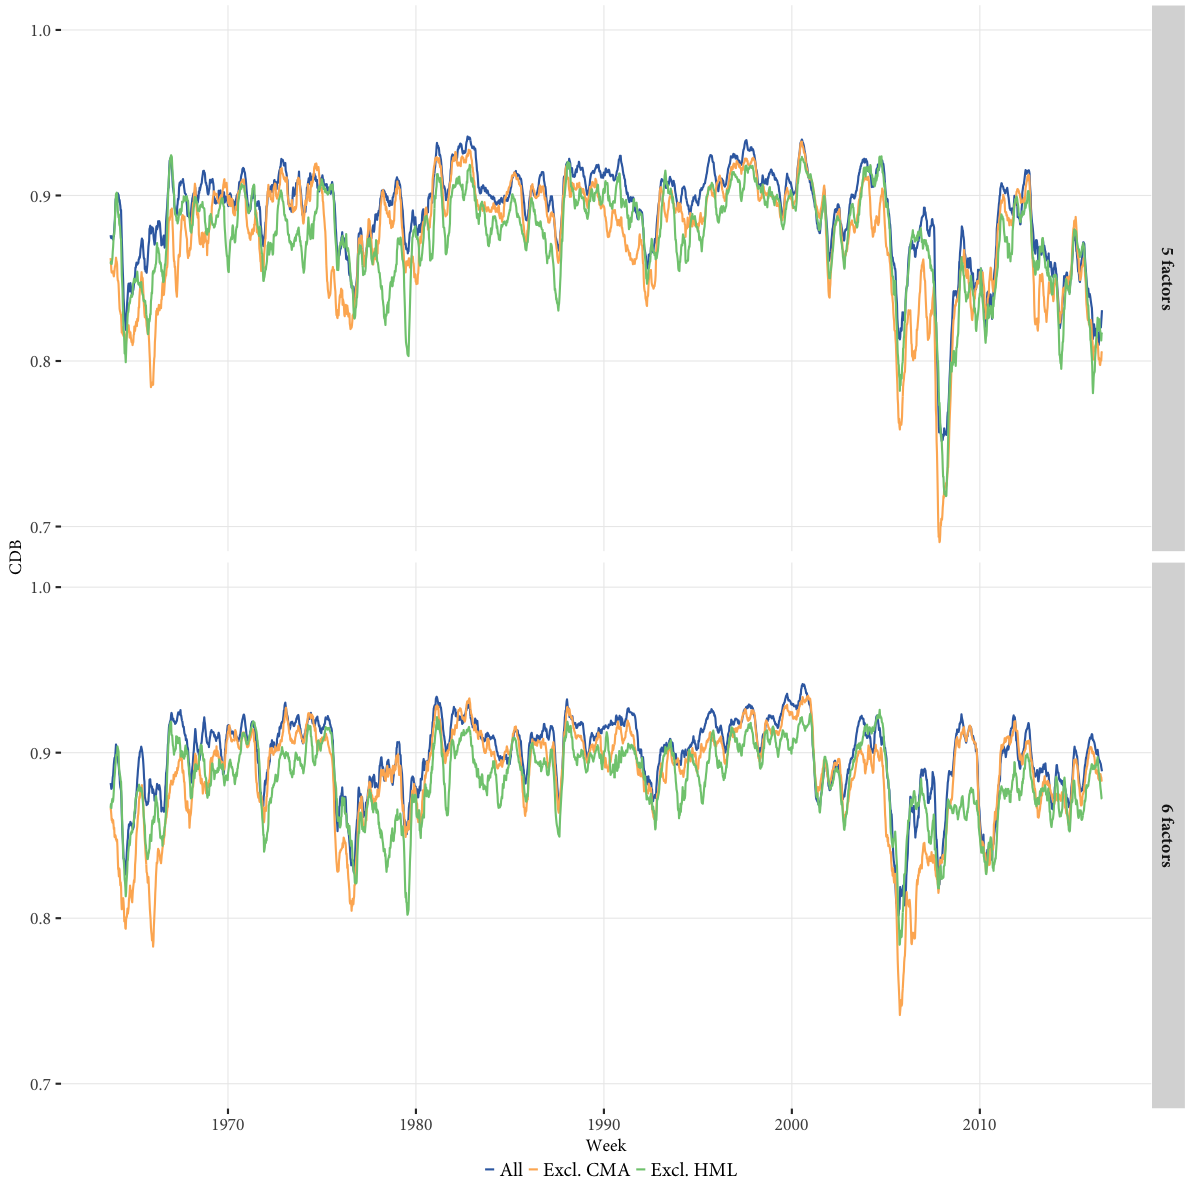
\includegraphics[scale = 1]{graphics/cdb_5F_6F.png}
\end{figure}

% CDB is very high; factor strategies are good diversifiers
First, we note that regardless of whether momentum is included or not, factor strategies appear to offer high levels of diversification. In absolute terms, all strategies fluctuate in the $0.80$ -- $0.95$ for the majority of the studied time period. 

% Dips
Second, there are notable dips in the diversification benefit measure. The dips represent times when diversification is relatively hard to come by, and roughly coincide in the five- and six-factor models. Interestingly, the periods of low diversification do not seem be stock market crises, as the CDB measure remains relatively high during the 1999-2000 bubble and the 2007-2009 recession.

% HML is a better diversifier on average
% CMA better when diversification is hard to come by
Third, the level decreases in diversification benefit of removing HML or CMA seem quite small. Furthermore, this decrease is highly similar; At certain times, portfolios including HML are more diversified and vice versa, but no pattern emerges. However, we note that the exclusion of RMW is dramatically different. Without RMW, the level decrease is substantial and dips in CDB become much more pronounced and frequent. 

[\autoref{tab:cdb_table} displays CDB summary statistics and the results of paired t-tests of the differences between strategies. This table tells the same story as the graph. Excluding RMW is significantly worse for diversification than excluding either HML or CMA. For HML and CMA, differences are small: In a five-factor setting [HML] is the significantly better diversifier, while in a six-factor setting [CMA] is. Although these differences are significant, we do not give much weight to them, as we have not accounted for the uncertainty in the estimation of the model that is the basis for the portfolio return distribution.]

In summary, we find that the high similarity of HML and CMA indicates that tail diversification benefits are not dramatically improved by including both the factors, which is coherent with fact that they are closely related and overlap. This does not mean that both factors should not be considered, however, as it could improve the conventional risk-return tradeoff in a mean-variance setting. The RMW factor, on the other hand, is shown to be very important for diversification purposes and should be considered by all factor investors concerned with tail risk.

%!TEX root = ../../main.tex

\begin{table}
  \centering
  \footnotesize
  \renewcommand{\arraystretch}{1.2}
  
  \caption{Conditional diversification benefit (CDB)\\ \quad \\
  Based on symmetric dynamic copula model, full sample (1963--2016). \emph{Difference} shows the average pair-wise difference in CDB between the column's and row's strategy, respectively, with t-test standard errors and significance levels (the first pair is thus the difference in pair-wise CDB between a five-factor strategy with and without CMA)}

  \begin{tabularx}{\textwidth}{@{} l X dddd X dd @{}}
    \toprule
    &&
      \multicolumn{4}{c}{CDB} && 
      \multicolumn{2}{c}{Difference} \\
    \cmidrule{3-6} \cmidrule{8-9}
    &&
      \multicolumn{1}{c}{Mean} &
      \multicolumn{1}{c}{SD} &
      \multicolumn{1}{c}{Min} &
      \multicolumn{1}{c}{Max} &&
      \multicolumn{1}{c}{All} &
      \multicolumn{1}{c}{Excl. CMA} \\
    \midrule
    \textbf{Five Factors} \\
    \emph{All}       && 88.937 & 3.410 & 61.469 & 95.135 &&   &                        \\
                     &&        &       &        &        &&   &                        \\
    \emph{excl. CMA} && 87.439 & 4.221 & 61.346 & 95.105 &&   1.497^{***} &             \\
                     &&        &       &        &        &&  (0.053)      &             \\
    \emph{excl. HML} && 87.448 & 3.731 & 61.722 & 94.274 &&   1.489^{***} & -0.009      \\
                     &&        &       &        &        &&  (0.050)      & (0.065)     \\
    \midrule
    \textbf{Six Factors} \\
    \emph{All}       && 89.783 & 2.898 & 72.850 & 95.043 &&   &                       \\
                     &&        &       &        &        &&   &                       \\
    \emph{excl. CMA} && 88.602 & 3.657 & 69.143 & 95.160 &&  1.181^{***} &             \\
                     &&        &       &        &        && (0.050)      &             \\
    \emph{excl. HML} && 88.259 & 3.053 & 71.987 & 94.447 &&  1.524^{***} &  0.343^{***}  \\
                     &&        &       &        &        && (0.049)      & (0.060)     \\
    \bottomrule
  \end{tabularx}

  \label{tab:cdb_table}
\end{table}


% What periods does low CDB correspond to?
% Story related to threshold correlations and patterns seen Mkt-HML

% No obvious corresponde with the market's performance. This does not appear
% to be related to the tail dependency so mcuh...

% subsection conditional_diversification_benefit (end)

\subsection{Diversification benefit in out-of-sample investing}

In an out-of-sample period covering one third of our available data, we now compare the diversification benefits under equal weights investing and mean-variance investing to the diversification benefits under the weights that give optimal CDB.

[We find that out-of-sample, the diversification benefits under mean-variance investing are in fact worse than equal weights investing. This indicates that equal weights investing is more robust in terms of tail diversification than mean-variance investing, and can explain why investors choose this method.]

